\documentclass[a4paper, 12pt, titlepage, fleqn]{article}

%Taal: Nederlands ("Inhoudsopgave", "Hoofdstuk",...)
\usepackage{graphicx}
\usepackage{subcaption}
\usepackage{amsmath, amssymb, textcomp, mathtools}
\usepackage{geometry}
	\geometry{a4paper, left=20mm, right=20mm, top=20mm, bottom=20mm}
\setlength{\mathindent}{1cm}
%Hyperlinks
\usepackage{hyperref}
\usepackage{subcaption}

%Opmaak hyperlinks
\hypersetup{colorlinks=false,	urlcolor=cyan,pdfborder=0 0 0}
\usepackage[framed,numbered,autolinebreaks,useliterate]{mcode}
%geen indents
\setlength\parindent{0pt}
\usepackage{listings}
\lstset{
language=Matlab, % choose the language of the code
%basicstyle=10pt, % the size of the fonts that are used for the code
numbers=left, % where to put the line-numbers
numberstyle=\footnotesize, % the size of the fonts that are used for the line-numbers
stepnumber=1, % the step between two line-numbers. If it's 1 each line will be numbered
numbersep=5pt, % how far the line-numbers are from the code
%backgroundcolor=\color{grey}, % choose the background color. You must add \usepackage{color}
showspaces=false, % show spaces adding particular underscores
showstringspaces=false, % underline spaces within strings
showtabs=false, % show tabs within strings adding particular underscores
frame=single, % adds a frame around the code
%tabsize=2, % sets default tabsize to 2 spaces
captionpos=b, % sets the caption-position to bottom
breaklines=true, % sets automatic line breaking
breakatwhitespace=false, % sets if automatic breaks should only happen at whitespace
escapeinside={\%*}{*)} % if you want to add a comment within your code
}

\captionsetup{
   font=small,          % Select font size
   margin=3em,          % Margin, left and right
   tableposition=top    % Formatting for captions above tables
}

\usepackage[dutch]{babel}
\begin{document}

\title{\textbf{Numerieke Modellering en Benadering: Chebyshev veeltermen}}
\author{Sander Prenen, r0701014}

\date{15 april 2020}
\begin{titlepage}
	\maketitle
	\thispagestyle{empty}
\end{titlepage}

\newpage
\tableofcontents
\newpage
\section{Inleiding}
In dit practicum worden de benaderingseigenschappen van Chebyshev veeltermen van de eerste soort bekeken. Deze veeltermen blijken uiterst geschikt voor het benaderen van eindige, re\"ele functies met behulp van de continue kleinste kwadratenbenadering. Ook zijn hun nulpunten vaak een uitstekende keuze voor de abscissa voor veelterminterpolatie. In sectie \ref{sec:benadering} wordt dieper ingegaan op de benaderingseigenschappen, terwijl in sectie \ref{sec:interpolatie} de interpolatie besproken wordt.

\section{Continue kleinste kwadratenbenadering met Chebyshev veeltermen}
\label{sec:benadering}
In deze sectie wordt geprobeerd continue functies op eindige, re\"ele intervallen te benaderen aan de hand van Chebyshev-veeltermen van de eerste soort. Dit zijn veeltermen die voldoen aan de volgende voorwaarde: $T_k(x) = \cos(k \cdot \arccos (x))$ voor $x \in [-1,1]$ en $k = 0,1,2,\ldots$ De veeltermen vormen een basis voor de ruimte $V_n$, een deelvectorruimte van $C([-1,1])$. 


\subsection{Beste benadering in $V_n$}
Indien de basisvectoren $T_k(x)$ orthogonale vectoren zijn, geldt volgende uitdrukking voor de beste benadering $y_n(x)$ voor een functie $f(x) \in C([-1,1])$:
\begin{equation}
y_n(x) = \sum_{k=0}^na_kT_k(x) \hspace{1cm} \text{met} \hspace{1cm} a_k = \frac{(f,T_k)}{(T_k,T_k)}
\label{eq:beste_benadering}
\end{equation}

Met als scalair product:
\begin{equation*}
(f,g) = \int_{-1}^1\frac{f(x)g(x)}{\sqrt{1-x^2}}dx
\end{equation*}

Om deze formule te kunnen gebruiken, moet dus worden aangetoond dat de basisvectoren orthogonaal zijn. Dit wil zeggen dat alle onderlinge scalaire producten nul zijn, behalve dat van een basisvector met zichzelf. Volgens bladzijde 69 in de cursus 'Numerieke modellering en benadering' van professor Vandewalle zijn de veeltermen wel degelijk ortohogonaal en mag de bovenstaande uitdrukking gebruikt worden. De resultaten van de scalaire prodcuten worden hier nog kort neergeschreven:
\begin{align}\label{eq:scalairProduct}
(T_k,T_j) = 
\begin{cases}
0,	& j \neq k\\
\frac{\pi}{2}, & j = k \neq 0\\
\pi, & j = k = 0
\end{cases}
\end{align}
%\subsubsection{Orthogonaliteit van de basisvectoren $T_k$}
%\label{subsec:scalaireProducten}
%In deze sectie wordt de orthogonaliteit van de basisvectoren bekeken. Hiervoor moeten alle onderlinge scalaire producten bepaald worden. Dit wordt gedaan uitgaande van drie gevallen:
%\begin{itemize}
%\item $k = l = 0$:
%\begin{equation*}
%(T_k,T_l) = \int_{-1}^1 \frac{T_0^2(x)}{\sqrt{1-x^2}}dx = \int_{-1}^1 \frac{1}{\sqrt{1-x^2}}dx =\left[\arcsin(x)\right]_{-1}^1 = \pi
%\end{equation*}
%\item $k = l \neq 0$:
%\begin{equation*}
%(T_k,T_l) = \int_{-1}^1\frac{T_k^2(x)}{\sqrt{1-x^2}}dx = \int_{-1}^1\frac{\cos^2(k \arccos(x))}{\sqrt{1-x^2}}dx = \frac{2\pi k + \sin(2\pi k)}{4k} = \frac{\pi}{2}
%\end{equation*}
%\item $k \neq l$:
%\begin{align*}
%(T_k,T_l) &= \int_{-1}^1\frac{T_k(x)T_l(x)}{\sqrt{1-x^2}}dx = \int_{-1}^1\frac{\cos(k \arccos(x))\cos(l \arccos(x))}{\sqrt{1-x^2}}dx\\
%&=\frac{1}{2}\int_{-1}^1\frac{\cos((k-l)\arccos(x))}{\sqrt{1-x^2}}dx + \frac{1}{2}\int_{-1}^1\frac{\cos((k+l)\arccos(x))}{\sqrt{1-x^2}}dx\\
%&=\frac{1}{2}\frac{\sin((k-l)\pi)}{k-l} + \frac{1}{2}\frac{\sin((k+l)\pi)}{k+l} = 0
%\end{align*}
%\end{itemize}
%Alle scalaire producten zijn nul, behalve die van basisvectoren met zichzelf. De vectoren zijn dus orthogonaal.

\subsubsection{Beste benadering}
Omdat de basisvectoren orthogonaal zijn, kan formule (\ref{eq:beste_benadering}) gebruikt worden. In deze sectie worden de co\"effici\"enten $a_k$ bepaald.
\begin{align*}
a_k &= \frac{(f,T_k)}{(T_k,T_k)} = \frac{1}{(T_k,T_k)}\int_{-1}^1\frac{f(x)T_k(x)}{\sqrt{1-x^2}}dx = \frac{1}{(T_k,T_k)}\int_{-1}^1\frac{f(x)\cos(k \arccos(x))}{\sqrt{1-x^2}}dx\\
&= \frac{1}{(T_k,T_k)}\int_\pi^0\frac{f(\cos \theta)\cos(k\theta)(-\sin(\theta))}{\sqrt{1-\cos^2(\theta)}}d\theta = \frac{1}{(T_k,T_k)}\int_0^\pi f(\cos \theta) cos(k\theta)d\theta
\end{align*}
Dit geeft dus volgende uitdrukking voor $a_k$, gebruikmakend van de uitdrukkingen in vergelijking~(\ref{eq:scalairProduct}):
\begin{align}
a_k = \begin{cases}
\frac{1}{\pi}\int_0^\pi f(\cos \theta)d\theta, & k = 0\\
\frac{2}{\pi}\int_0^\pi f(\cos \theta)\cos(k\theta)d\theta, & k > 0
\end{cases}
\label{eq:a_K}
\end{align}



\subsection{Evalueren van de Chebyshev veeltermen}
Om de beste benadering numeriek te bepalen, moet vergelijking (\ref{eq:beste_benadering}) ge\"evalueerd worden. De functie \texttt{evalCheb} geeft een vector $v = (f_1, f_2, \ldots, f_N) \in \mathbb{R}^N$ terug. Deze vector wordt bekomen uit inputvectoren $a = (a_0,a_1,\ldots, a_n) \in \mathbb{R}^{n+1}$ en $x = (x_1,x_2,\ldots,x_N) \in \mathbb{R}^N$ op de volgende manier:
\begin{equation*}
f_i = y_n(x_i) = a_0T_0(x_i) + a_1T_1(x_i) + \ldots + a_nT_n(x_i)
\end{equation*}

In Listing \ref{lst:evalCheb} wordt de MATLAB code voor deze berekening weergegeven.

\lstinputlisting[caption={evalCheb.m}, label = {lst:evalCheb}]{../evalCheb.m}


\subsection{Bepalen van de co\"effici\"enten}
Voor het bepalen van de co\"effici\"enten $a_k$ kan vergelijking (\ref{eq:a_K}) gebruikt worden. Deze vergelijking kan met behulp van de trapeziumregel voor numerieke integratie met een discretizatie bestaande uit $n$ intervallen, benaderd worden door:
\begin{align*}
a_k \approx \frac{1}{n}f(1) + \frac{2}{n}\sum_{l=1}^{n-1}f\left(\cos\left(\frac{l\pi}{n}\right)\right)\cos\left(k\frac{l\pi}{n}\right) + \frac{(-1)^k}{n}f(-1), \hspace{1cm} 0 < k \leq n
\end{align*}
Hieruit volgt dat de co\"effici\"enten $a_k$ kunnen berekend worden als de discrete cosinus transformatie (DCT) van de rij:
\begin{align}
f(z_{0,n}),f(z_{1,n}), \ldots, f(z_{n,n})
\label{eq:DCTrij}
\end{align} 
Hierin is $z_{l,n} = \cos(l\pi/n)$. Deze punten zijn de extrema van $T_k(x)$ aangezien dit de nulpunten zijn van de eerste afgeleide van $T_k(x)$.

\begin{align*}
\frac{dT_k(x)}{dx} &= \frac{d}{dx}\cos(k\arccos(x)) = -\sin(k \arccos(x))\cdot k \cdot - \frac{1}{\sqrt{1-x^2}}
\end{align*}

De afgeleide wordt nul als $k=0$ of $\sin(k \arccos(x)) = 0$. In het tweede geval herleidt dit zich tot:
\begin{align*}
k\arccos(x) = l\pi \Leftrightarrow x = \cos\left(\frac{l\pi}{k}\right)
\end{align*}

In de functie \texttt{approxCheby} wordt de DCT van de rij in vergelijking (\ref{eq:DCTrij}) bepaald. De code van deze functie kan gevonden worden in Listing \ref{lst:approxCheby}.
\lstinputlisting[caption={approxCheby.m}, label = {lst:approxCheby}]{../approxCheby.m}


\subsection{Benaderen van een functie}
De algoritmes die in Listing \ref{lst:evalCheb} en \ref{lst:approxCheby} te zien zijn, kunnen gebruikt worden voor het benaderen van een willekeurige functie in $C([-1,1])$. Om een functie te benaderen worden de co\"effici\"enten $a_k$ bepaald met \texttt{approxCheby}. Deze co\"effici\"enten worden meegegeven aan \texttt{evalCheb}. De punten waarin de benadering ge\"evalueerd moet worden, worden meegegeven in de $x$ vector. In dit geval wordt gekozen voor 200 equidistante punten tussen $-1$ en $1$.

In figuur \ref{fig:rungeFunctie} worden de beste benaderingen voor de Runge functie in ruimtes $V_2$ tot $V_{20}$ weergegeven. De Runge functie heeft als voorschrift $f(x) = \frac{1}{25x^2+1}$. Figuur \ref{fig:rungeFoutBenadering} toont de maximale afwijking $d(y_n,f) = \max_{x \in [-1,1]}|y_n(x)-f(x)|$, in functie van de graad $n$ van de benaderende veelterm.  Deze fout daalt exponentieel met stijgende $n$. Merk op dat deze afstand niet de ge\"induceerde afstand van het scalair product is.
\begin{figure}[h]
\centering
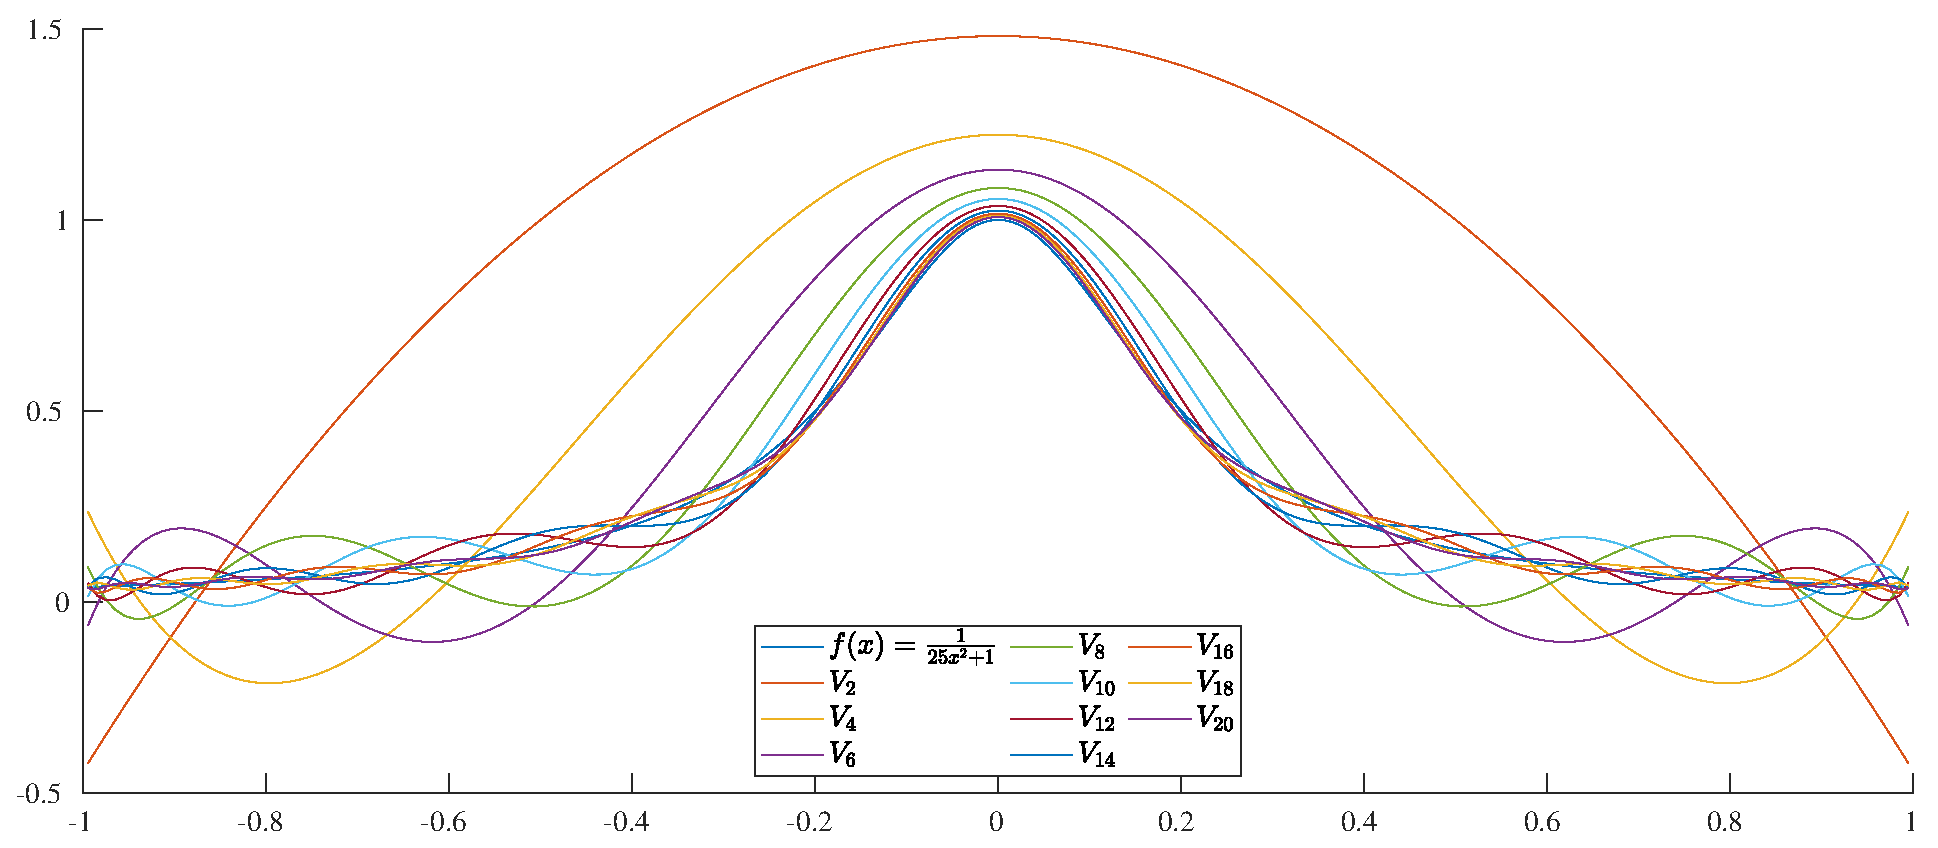
\includegraphics[scale=0.4]{../Afbeeldingen/rungeBenadering.eps}
\caption{De beste benaderingen van de Runge functie in de ruimtes $V_2$ tot $V_{20}$.
\label{fig:rungeFunctie}}
\end{figure}

\begin{figure}
\centering
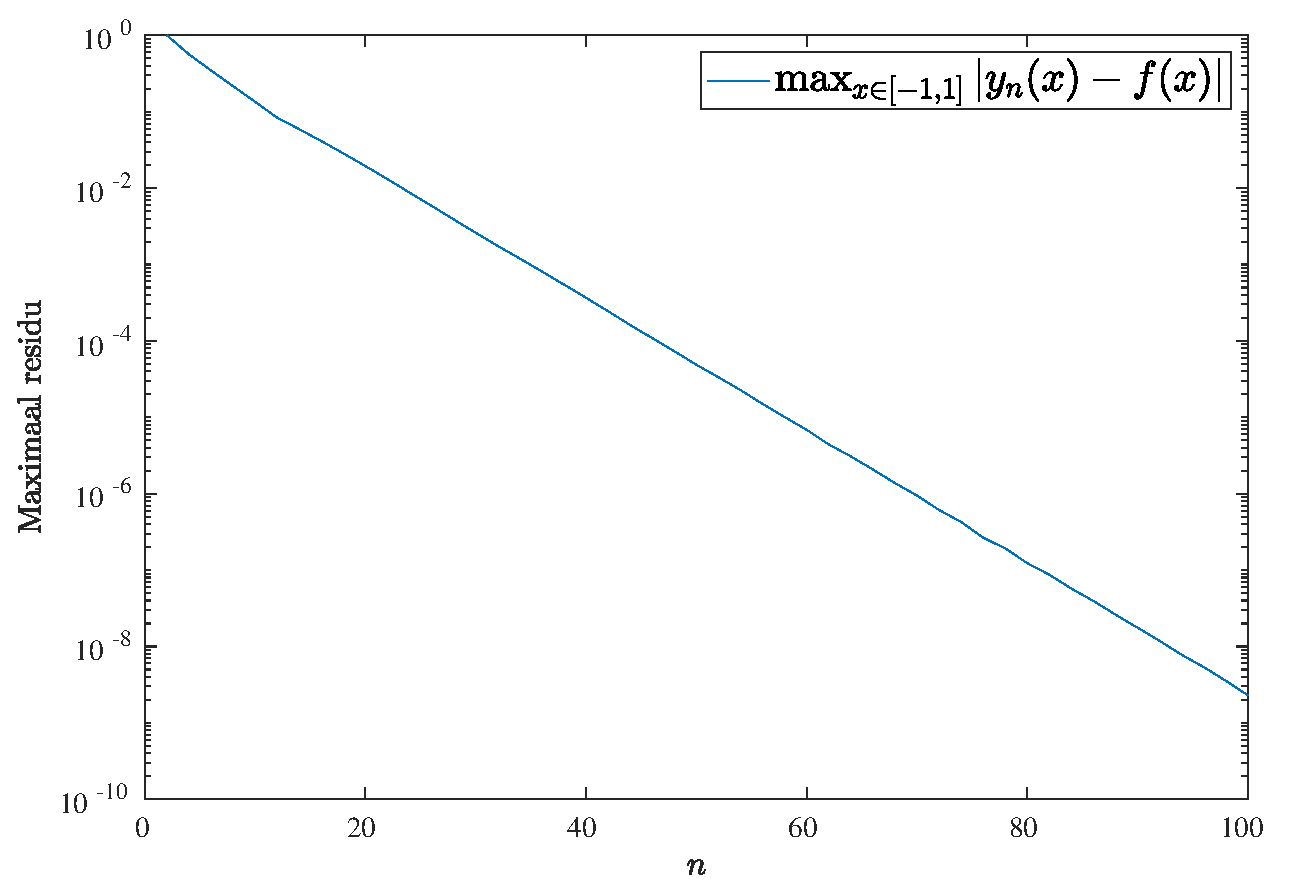
\includegraphics[scale=0.4]{../Afbeeldingen/rungeFout.eps}
\caption{De maximale fout voor de benadering van de runge functie in de ruimtes $V_2$ tot $V_{100}$.
\label{fig:rungeFoutBenadering}}
\end{figure}

\section{Interpolatie in Chebyshev knooppunten}
\label{sec:interpolatie}
Veeltermen van graad $n-1$ kunnen een functie interpoleren in $n$ interpolatiepunten. De interpolatiepunten $x_k$, voor $k = 1,2,\ldots,n$, kunnen vrij gekozen worden. Er wordt gezocht naar een veelterm $g(x)$ van graad $n-1$ die de functie $f(x)$ interpoleert, zodanig dat de volgende voorwaarde voldaan is:
\begin{align*}
g(x_i) = f(x_i), \hspace{1cm} i = 1,\ldots,n
\end{align*}
De veelterm $g(x)$ kan worden voorgesteld in de vorm $g(x) = \sum_{k=0}^{n-1}c_k\psi_k(x)$. Hierin zijn $\psi_k(x)$ de basisfuncties, in dit geval dus $T_k(x)$. De interpolatievoorwaarden leiden tot volgend lineair stelsel:
\begin{align}
Mc = B
\label{eq:matrixM}
\end{align}
De oplossing van dit stelsel is de vector $c$ met de co\"effici\"enten $c_k$. De elementen $M_{ij}$ van de matrix $M$ op rij $i$ en kolom $j$ worden gegeven door:
\begin{align*}
M_{ij} = \psi_j(x_i) = T_j(x_i)
\end{align*}
en de elementen $B_i$ van de vector $B$ worden gegeven door:
\begin{align*}
B_i = f(x_i).
\end{align*}

In de functie \texttt{interpolate} worden de co\"effici\"enten $c_k$ en het conditiegetal van de matrix $M$ berekend. Als invoer verwacht de functie de interpolatiepunten $x_k$ en de te benaderen functie~$f(x)$. De code van deze functie is terug te vinden in Listing \ref{lst:interpolate}.

\lstinputlisting[caption={interpolate.m}, label = {lst:interpolate}]{../interpolate.m}

\subsection{Interpoleren van een functie}
\subsubsection{Cosinus functie interpoleren}
\label{cosInterpoleren}
De functie \texttt{interpolate} wordt gebruikt om de functie $f(x) = \cos(x)$ te benaderen. De co\"effici\"enten $c_k$ worden meegegeven aan de functie \texttt{evalCheb} om de interpolant $g(x)$ te kunnen plotten. Voor de interpolatiepunten $x_k$ worden eerst equidistante punten gekozen. De resultaten worden voor verschillende $n$-waarden getoond in figuren \ref{lageNCosEqui} en \ref{fig:hogeNCosEqui}. Naarmate $n$ stijgt vertoont de benadering aan de randen meer afwijking ten op zichte van $f(x)$. Bij een te hoge $n$ zoals in figuur \ref{fig:hogeNCosEqui} is de benadering aan de rand heel slecht doordat de gebruikte methode niet stabiel is bij equidistante interpolatiepunten. Echter wordt de benadering in het midden steeds beter. Door de interpolatiepunten zo te kiezen dat ze de nulpunten zijn van de $k$-de Chebyshev veelterm, wordt de methode wel stabiel. Deze nulpunten zijn van de vorm:
\begin{align*}
x_i = \cos\left(\frac{\pi(2i-1)}{2k}\right), \hspace{1cm} i = 1,\ldots,k
\end{align*}
Deze punten worden ook wel de Chebyshev knooppunten genoemd. In figuren \ref{fig:lageNCosNul} en \ref{fig:hogeNCosNul} zijn de interpolatieveeltermen met de Chebyshev knooppunten te zien. De fouten aan de randen zijn veel kleiner en zelfs voor hoge $n$ waarden is de methode stabiel. Dit kan gezien worden in figuur~\ref{fig:hogeNCosNul}.


\begin{figure}
\centering
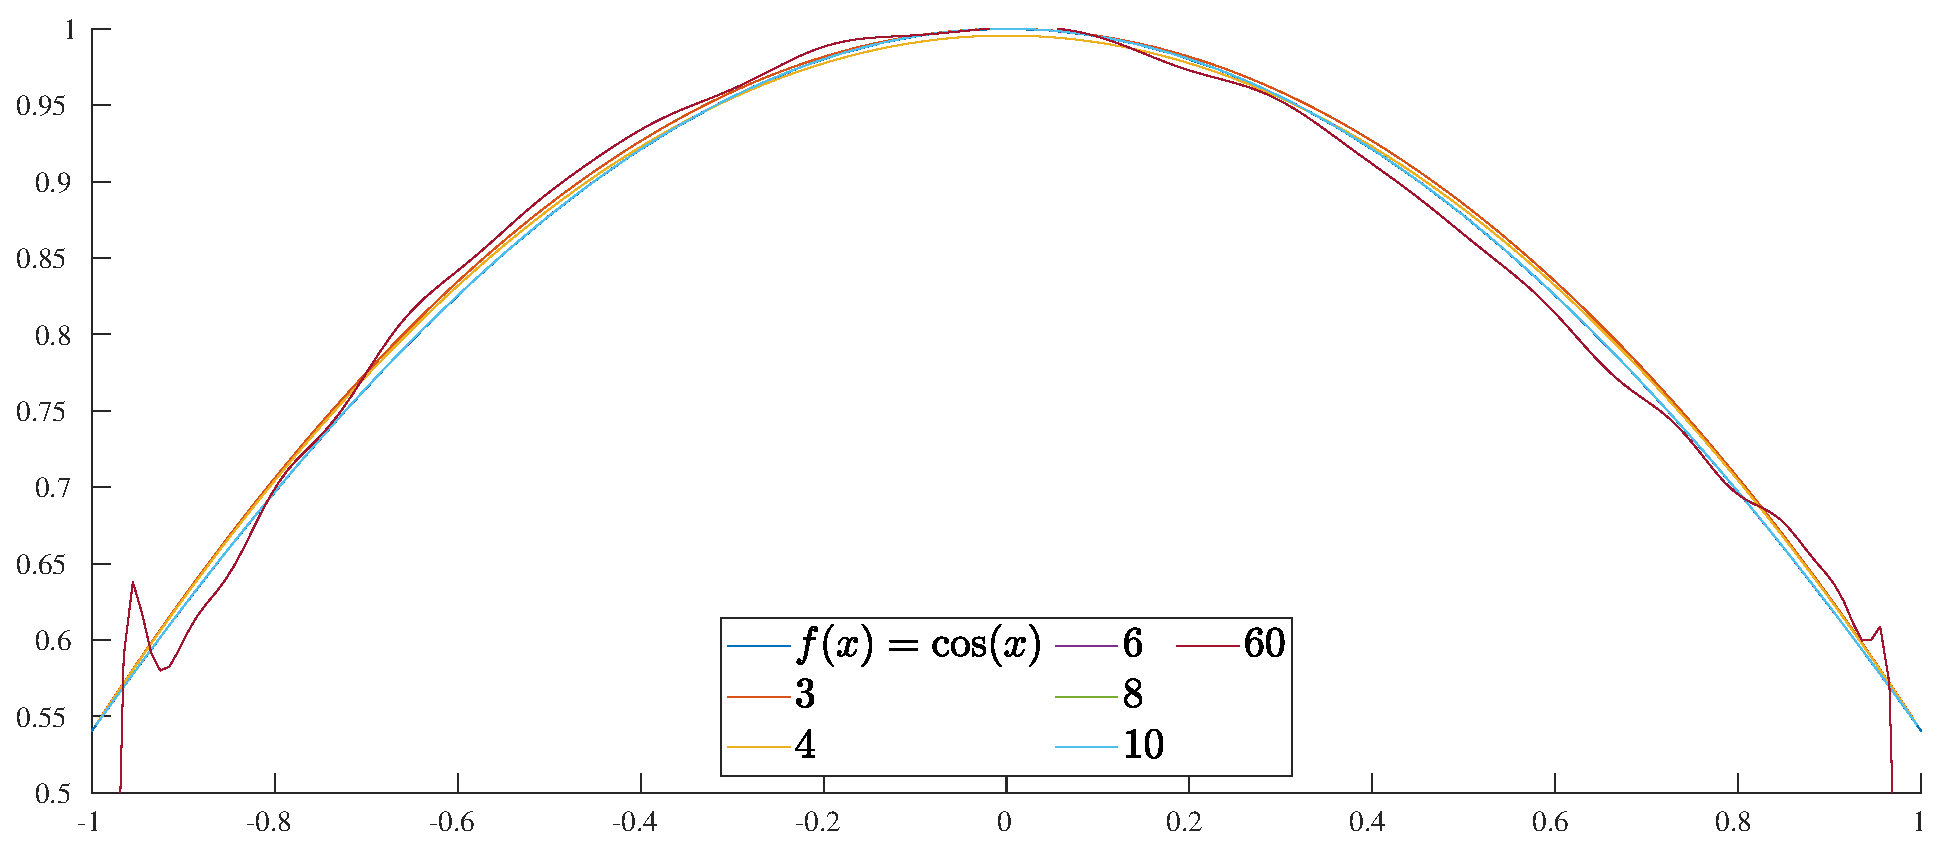
\includegraphics[scale=0.4]{../Afbeeldingen/cos_equi_laag.eps}
\caption{Interpolatie van de functie $f(x) = \cos(x)$ met een lage $n$ en equidistante interpolatiepunten. De cijfers in de legende zijn de verschillende $n$-waarden.}
\label{lageNCosEqui}
\end{figure}

\begin{figure}
\centering
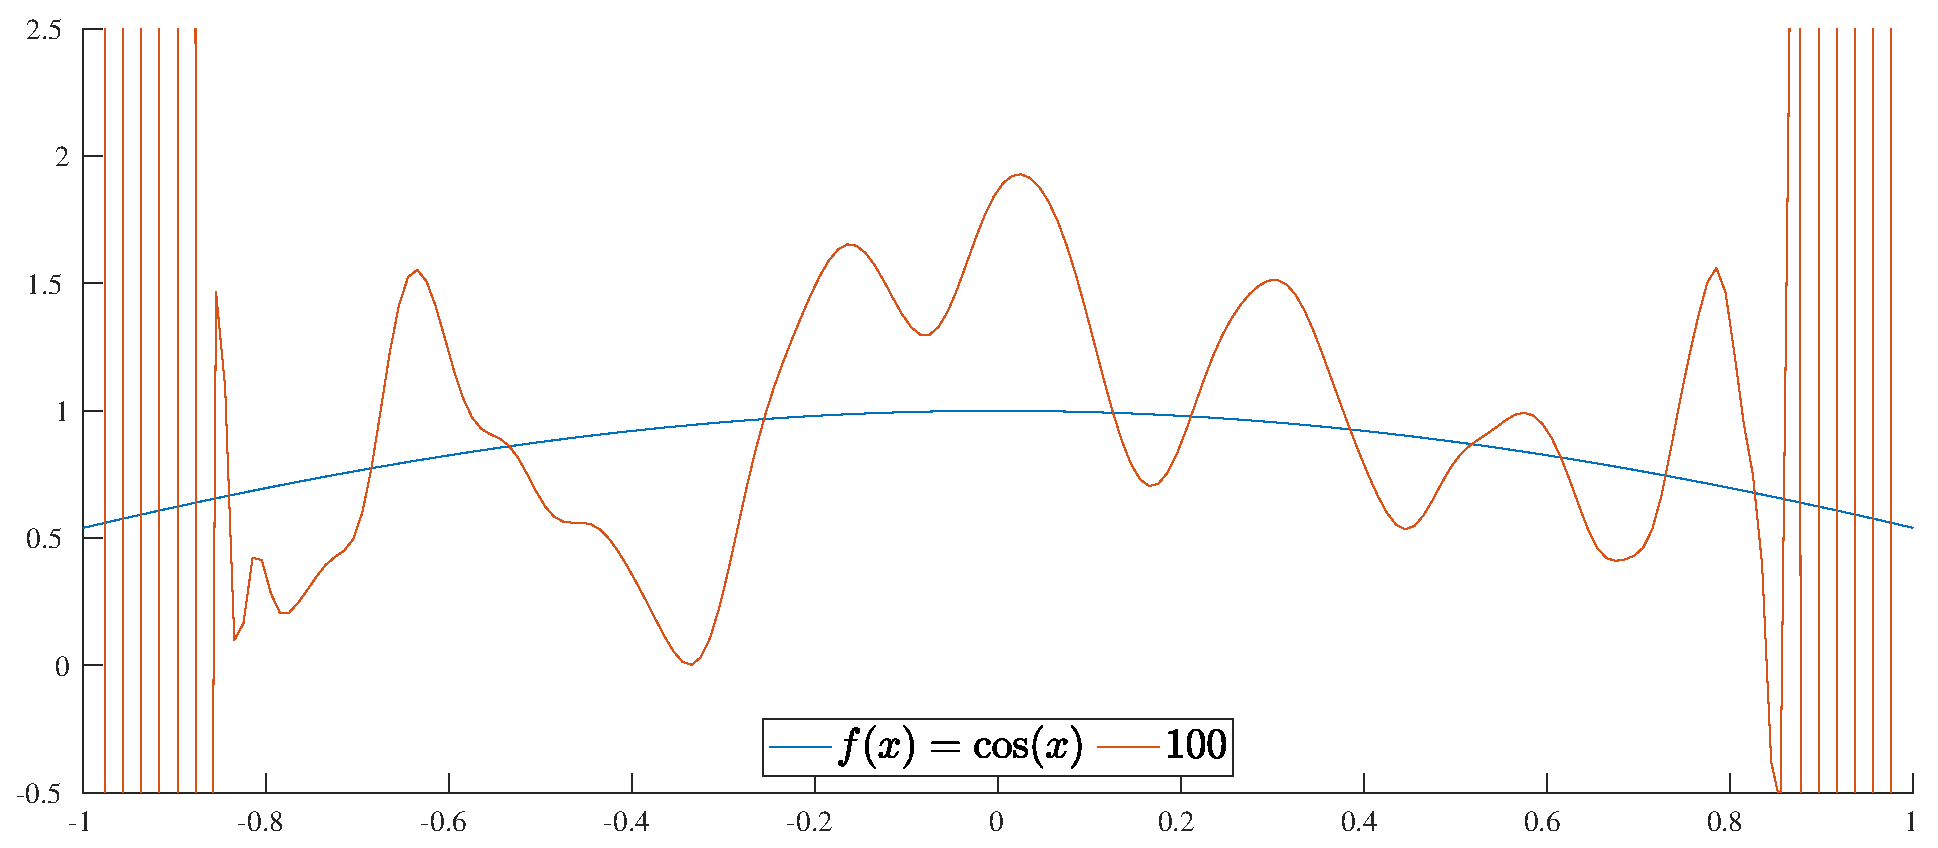
\includegraphics[scale=0.4]{../Afbeeldingen/cos_equi_hoog.eps}
\caption{Interpolatie van de functie $f(x) = \cos(x)$ met een hoge $n$ en equidistante interpolatiepunten. De cijfers in de legende zijn de verschillende $n$-waarden.}
\label{fig:hogeNCosEqui}
\end{figure}

\begin{figure}
\centering
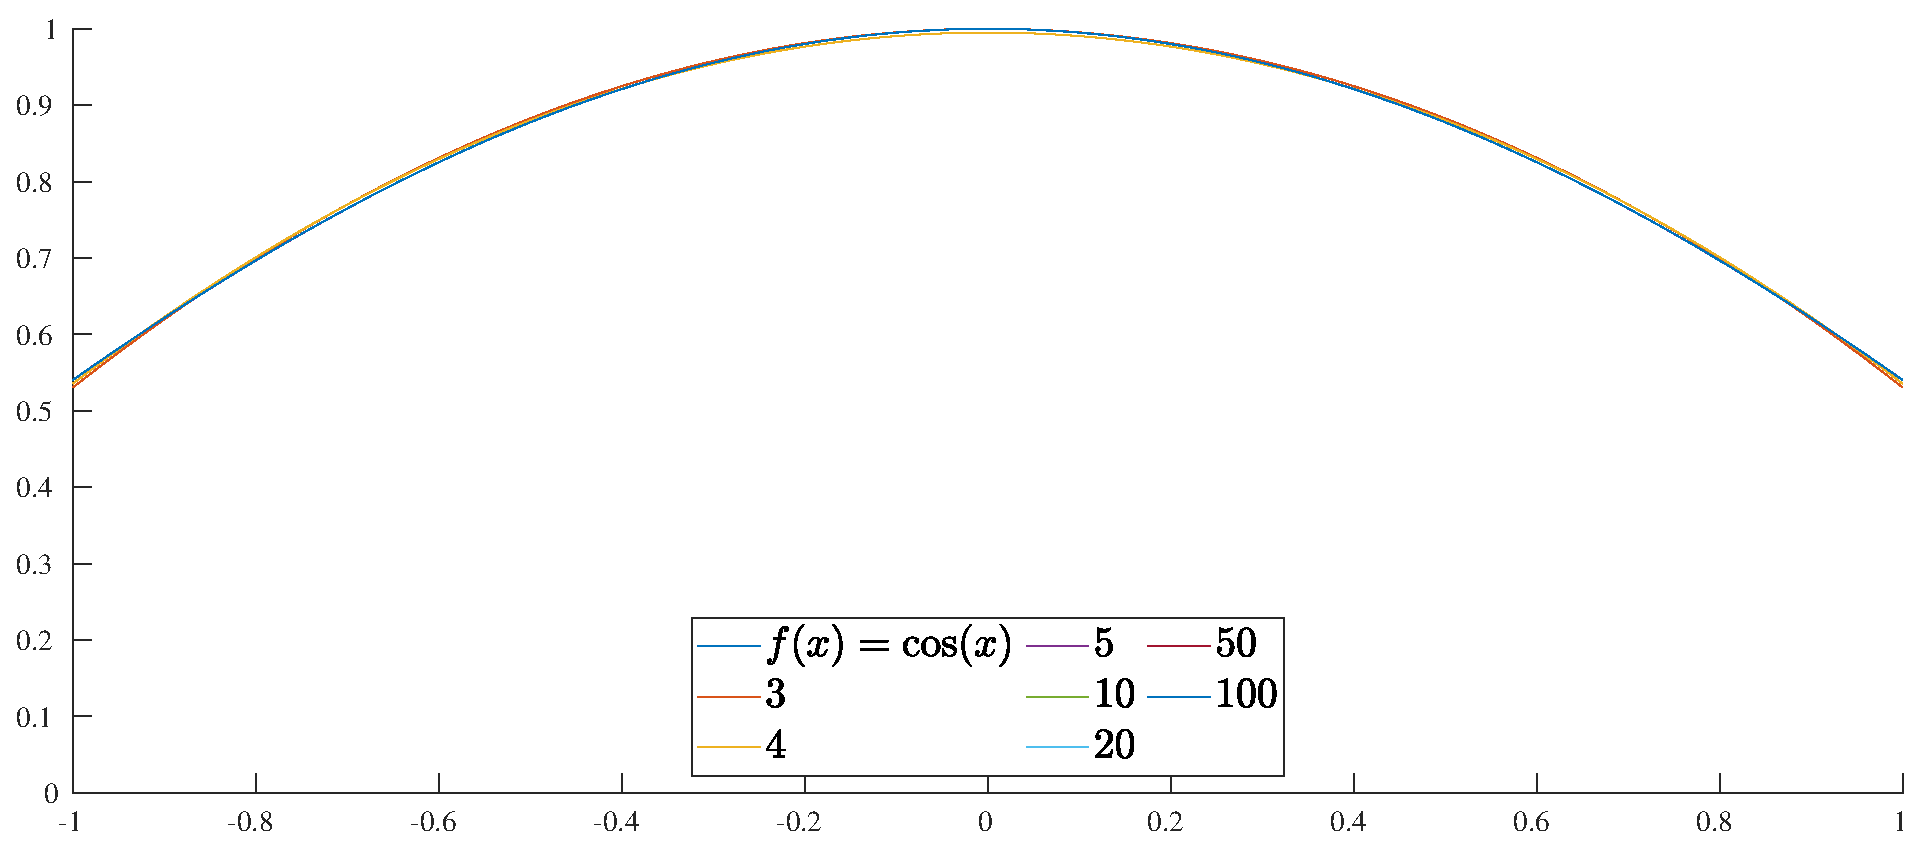
\includegraphics[scale=0.4]{../Afbeeldingen/cos_nul_laag.eps}
\caption{Interpolatie van de functie $f(x) = \cos(x)$ met een lage $n$ en Chebyshev knooppunten. De cijfers in de legende zijn de verschillende $n$-waarden.}
\label{fig:lageNCosNul}
\end{figure}

\begin{figure}
\centering
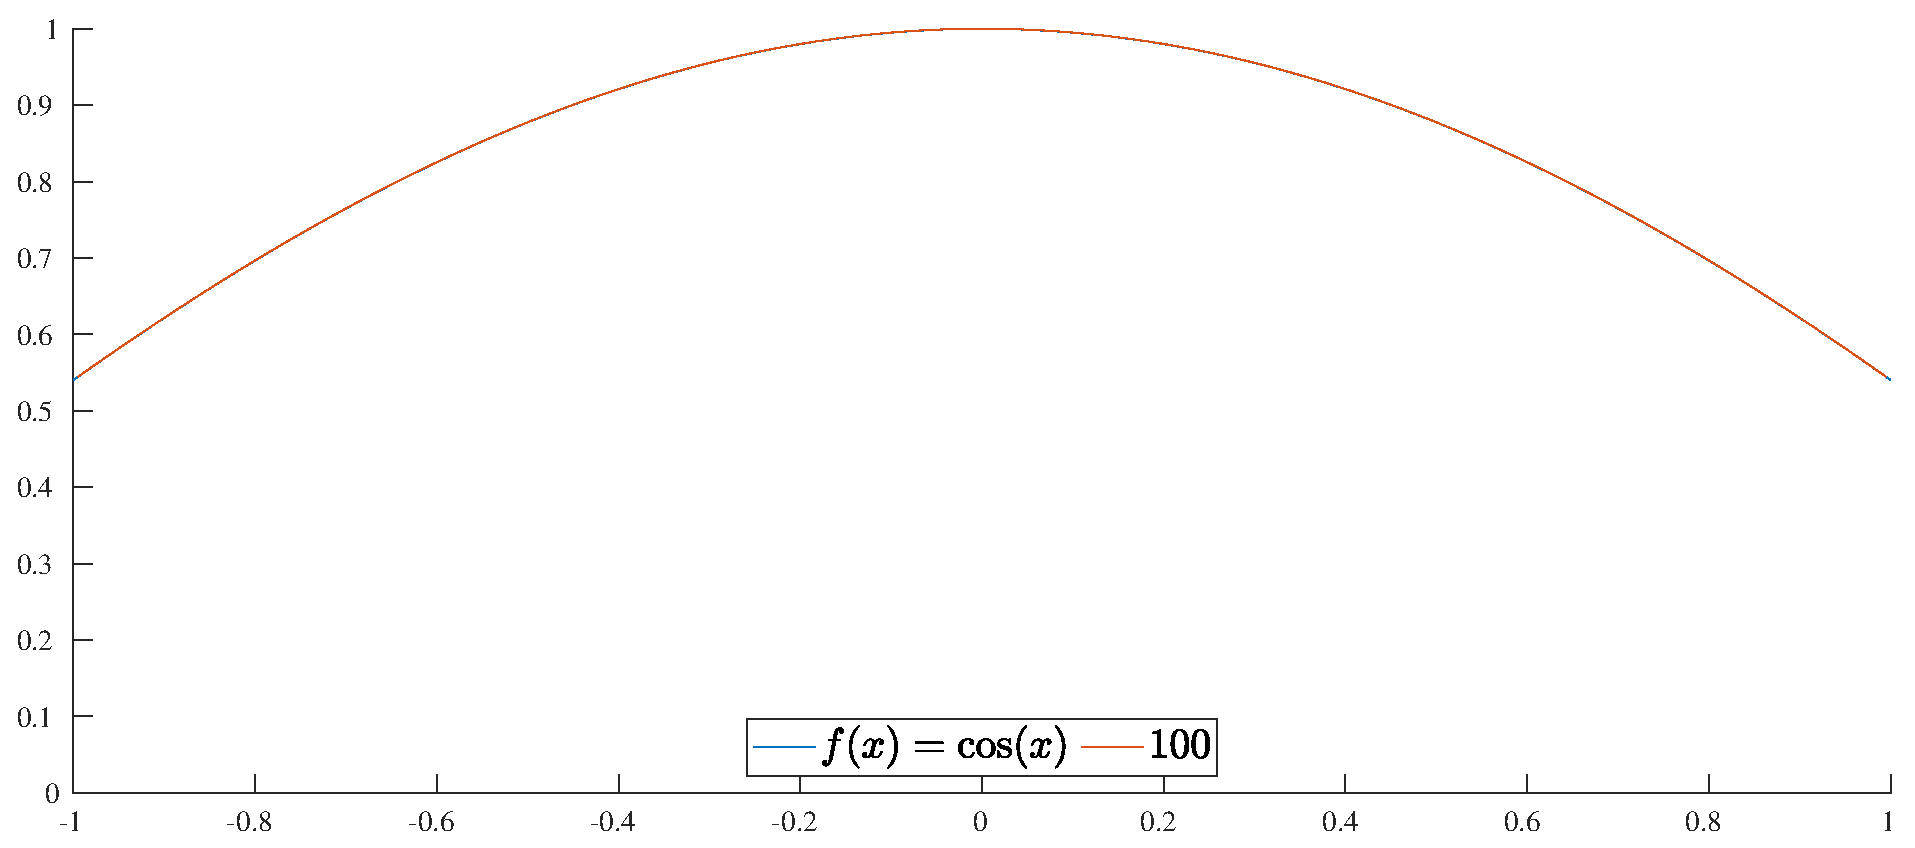
\includegraphics[scale=0.4]{../Afbeeldingen/cos_nul_hoog.eps}
\caption{Interpolatie van de functie $f(x) = \cos(x)$ met een hoge $n$ en Chebyshev knooppunten. De cijfers in de legende zijn de verschillende $n$-waarden.}
\label{fig:hogeNCosNul}
\end{figure}

\newpage
\subsubsection{Runge functie interpoleren}
Met eenzelfde werkwijze als in sectie \ref{cosInterpoleren} wordt nu de runge functie $f(x) = \frac{1}{25x^2+1}$ ge\"interpoleerd. Eerst worden equidistante interpolatiepunten $x_k$ gebruikt. Deze resultaten zijn te zien in figuren~\ref{fig:lageNRungeEqui} en \ref{fig:hogeNRungeEqui}. De fout aan de randen wordt groter bij een stijgende waarde van $n$, maar de benadering in het midden van het interval wordt beter.  Opnieuw kunnen als interpolatiepunten ook de Chebyshev knooppunten gebruikt worden. Hierdoor wordt de methode stabiel en verdwijnen de fouten aan de randen. De resultaten van deze interpolaties kunnen in figuren \ref{fig:lageNRungeNul} en \ref{fig:hogeNRungeNul} bekeken worden.

\begin{figure}
\centering
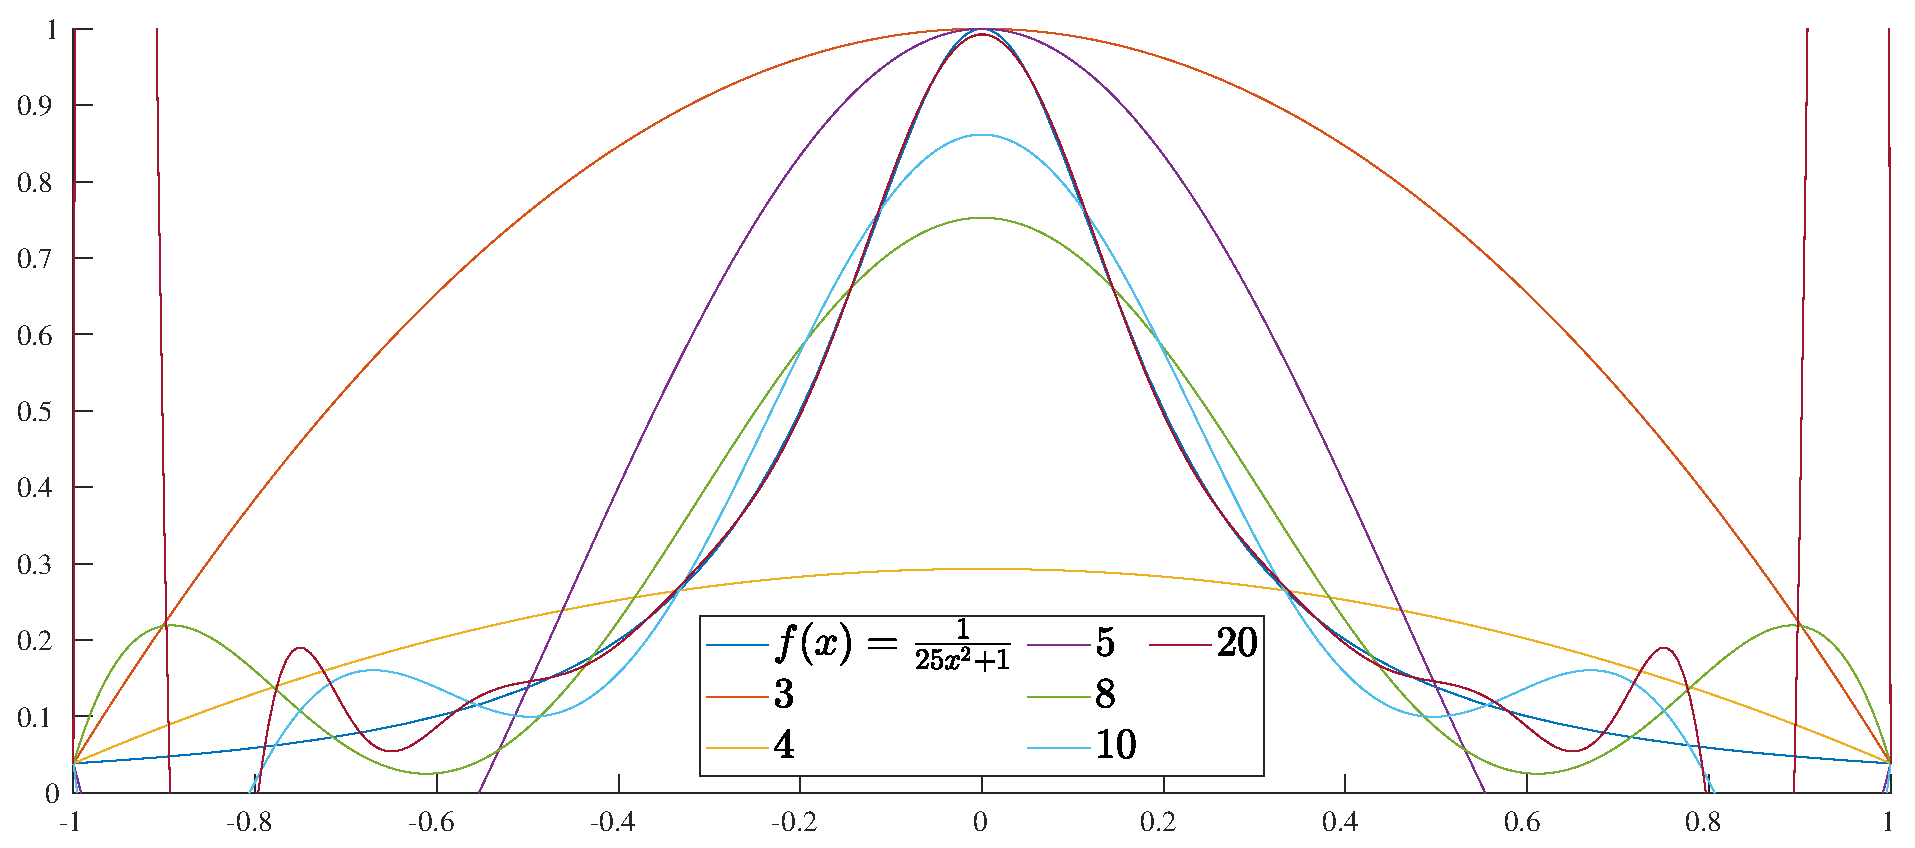
\includegraphics[scale=0.4]{../Afbeeldingen/runge_equi_laag.eps}
\caption{Interpolatie van de functie $f(x) = \frac{1}{25x^2+1}$ met een lage $n$ en equidistante interpolatiepunten. De cijfers in de legende zijn de verschillende $n$-waarden.}
\label{fig:lageNRungeEqui}
\end{figure}

\begin{figure}
\centering
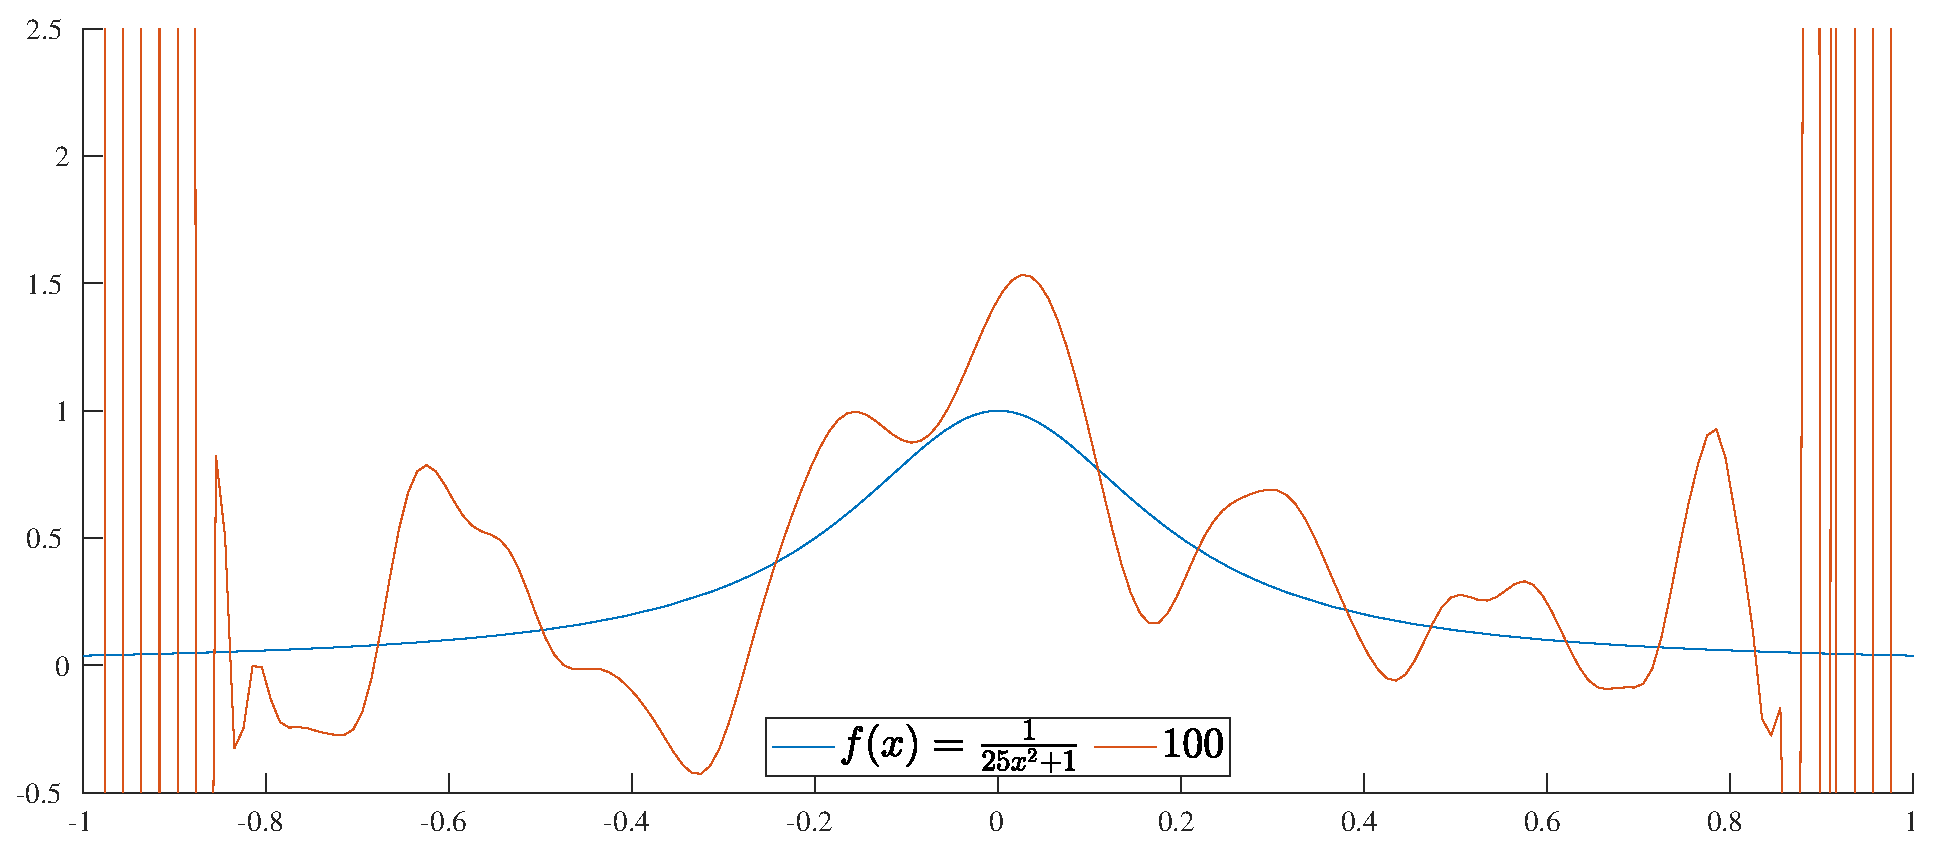
\includegraphics[scale=0.4]{../Afbeeldingen/runge_equi_hoog.eps}
\caption{Interpolatie van de functie $f(x) = \frac{1}{25x^2+1}$ met een hoge $n$ en equidistante interpolatiepunten. De cijfers in de legende zijn de verschillende $n$-waarden.}
\label{fig:hogeNRungeEqui}
\end{figure}

\begin{figure}
\centering
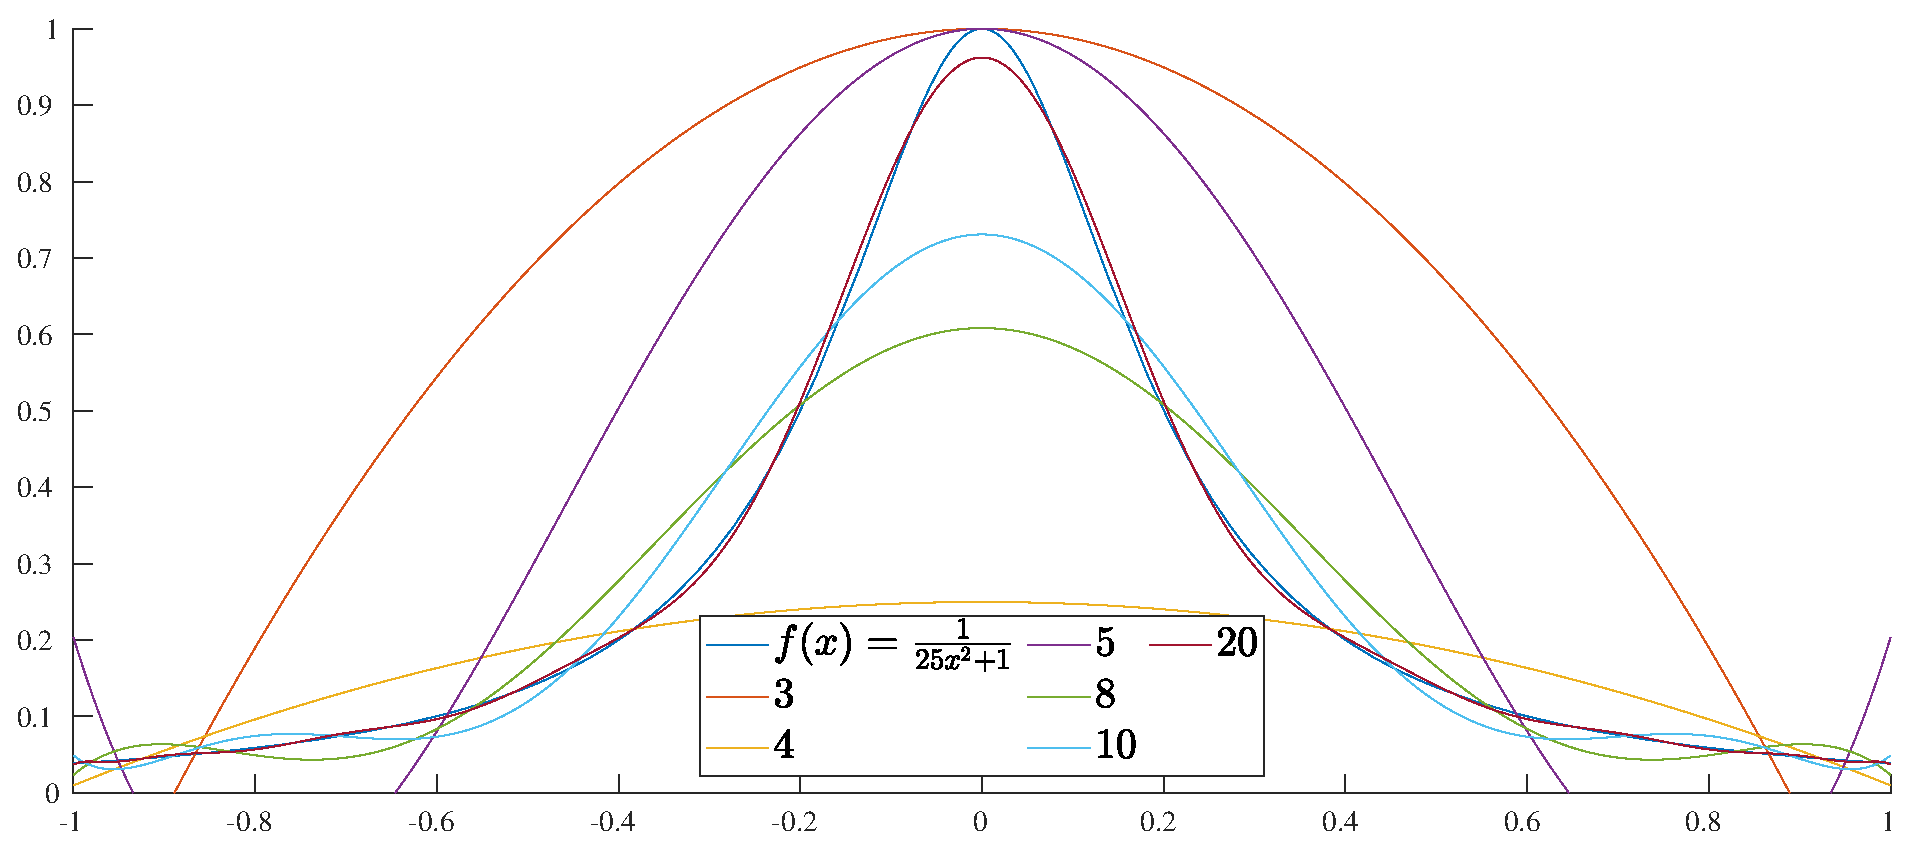
\includegraphics[scale=0.4]{../Afbeeldingen/runge_nul_laag.eps}
\caption{Interpolatie van de functie $f(x) = \frac{1}{25x^2+1}$ met een lage $n$ en Chebyshev knooppunten. De cijfers in de legende zijn de verschillende $n$-waarden.}
\label{fig:lageNRungeNul}
\end{figure}

\begin{figure}
\centering
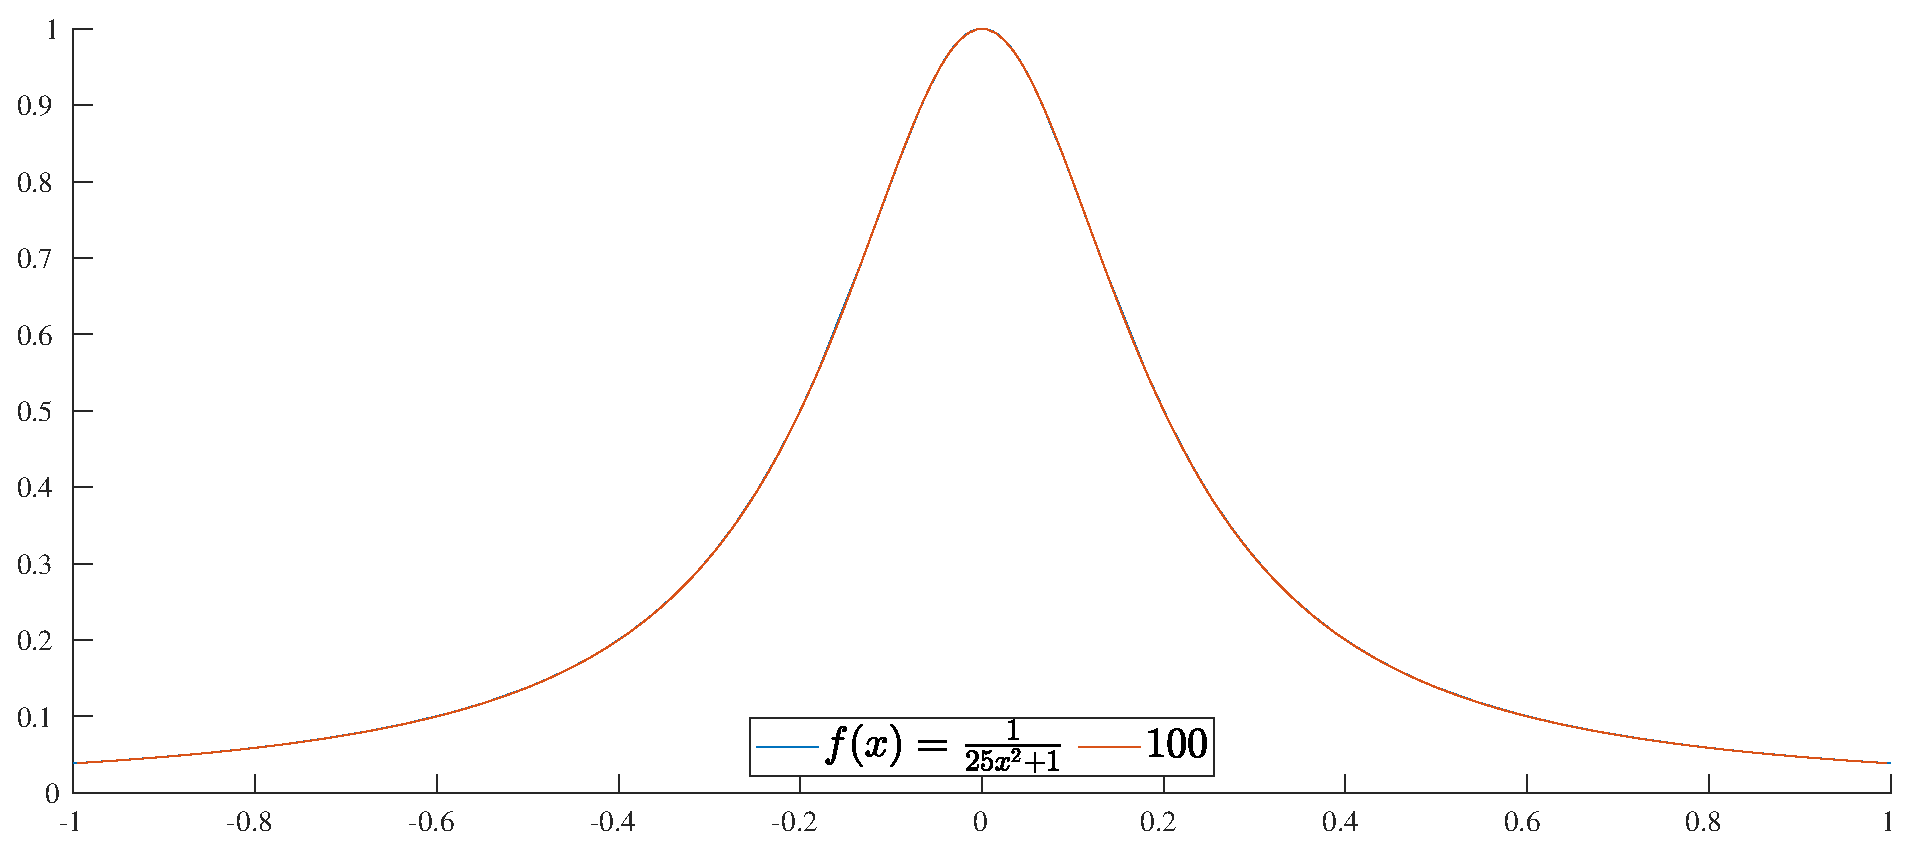
\includegraphics[scale=0.4]{../Afbeeldingen/runge_nul_hoog.eps}
\caption{Interpolatie van de functie $f(x) = \frac{1}{25x^2+1}$ met een hoge $n$ en Chebyshev knooppunten. De cijfers in de legende zijn de verschillende $n$-waarden.}
\label{fig:hogeNRungeNul}
\end{figure}

\newpage
\subsubsection{Grootte van de fouten en conditie van de matrix $M$}
In figuur \ref{fig:cosHeleFout} en figuur \ref{fig:rungeHeleFout} wordt de fout over het hele interval $[-1,1]$ voor verschillende waarden van $n$ geplot. Er kan duidelijk gezien worden dat voor equidistante interpolatiepunten de fouten zich vooral voordoen aan de randen en dat deze fout groter wordt met stijgende $n$. Voor de Chebyshev-interpolatiepunten is de fout in het midden groter in vergelijking met de randen. Dit is te wijten aan de ligging van de interpolatiepunten. Er liggen meer punten bij de randen waardoor de benadering er beter is. Dit effect is goed te zien op de vijfde plot van figuur \ref{fig:rungeHeleFout}.
In figuren \ref{fig:cosFout} en \ref{fig:rungeFout} wordt de maximale afwijking $d(g,f) = \max_{x\in [-1,1]} | g(x) - f(x)|$, in functie van het aantal interpolatiepunten geschetst. Voor equidistante interpolatiepunten daalt de fout eerst, maar door de instabiliteit van de methode zal vanaf een grotere $n$ de fout weer stijgen. Als de Chebyshev knooppunten als interpolatiepunten worden gekozen dan is de fout monotoon dalend tot de machineprecisie. De zaagtandstructuur die te zien is in figuur \ref{rungeNulFout} is te wijten aan de vorm van de runge functie. Bij een oneven aantal interpolatiepunten, ligt er een interpolatiepunt in het midden van het interval. Hierdoor zal de piek van de runge functie beter benaderd worden en is de fout bijgevolg kleiner.
 
Dat de gebruikte methode instabiel is, kan ook afgeleid worden uit het conditiegetal $\kappa$ van de matrix $M$ in vergelijking (\ref{eq:matrixM}). Dit getal geeft weer hoe het resultaat van een bewerking verandert met de invoer. Hoe hoger het conditiegetal, hoe groter de afwijking op het resultaat zal zijn bij een kleine afwijking van de invoer. In figuur \ref{fig:kappa} is te zien hoe het conditiegetal $\kappa$ van de matrix $M$ evolueert in functie van het aantal interpolatiepunten $n$. Bij een equidistante verdeling van de interpolatiepunten, neemt $\kappa$ al snel een heel grote waarde aan, hetgeen de instabiliteit van de methode verklaart. Indien de nulpunten van de $k$-de Chebyshev veelterm gebruikt worden om te interpoleren, blijft $\kappa$ een constante, lage waarde onafhankelijk van $n$. Dit verklaart waarom met deze interpolatiepunten de methode wel stabiel is.

\begin{figure}
\centering
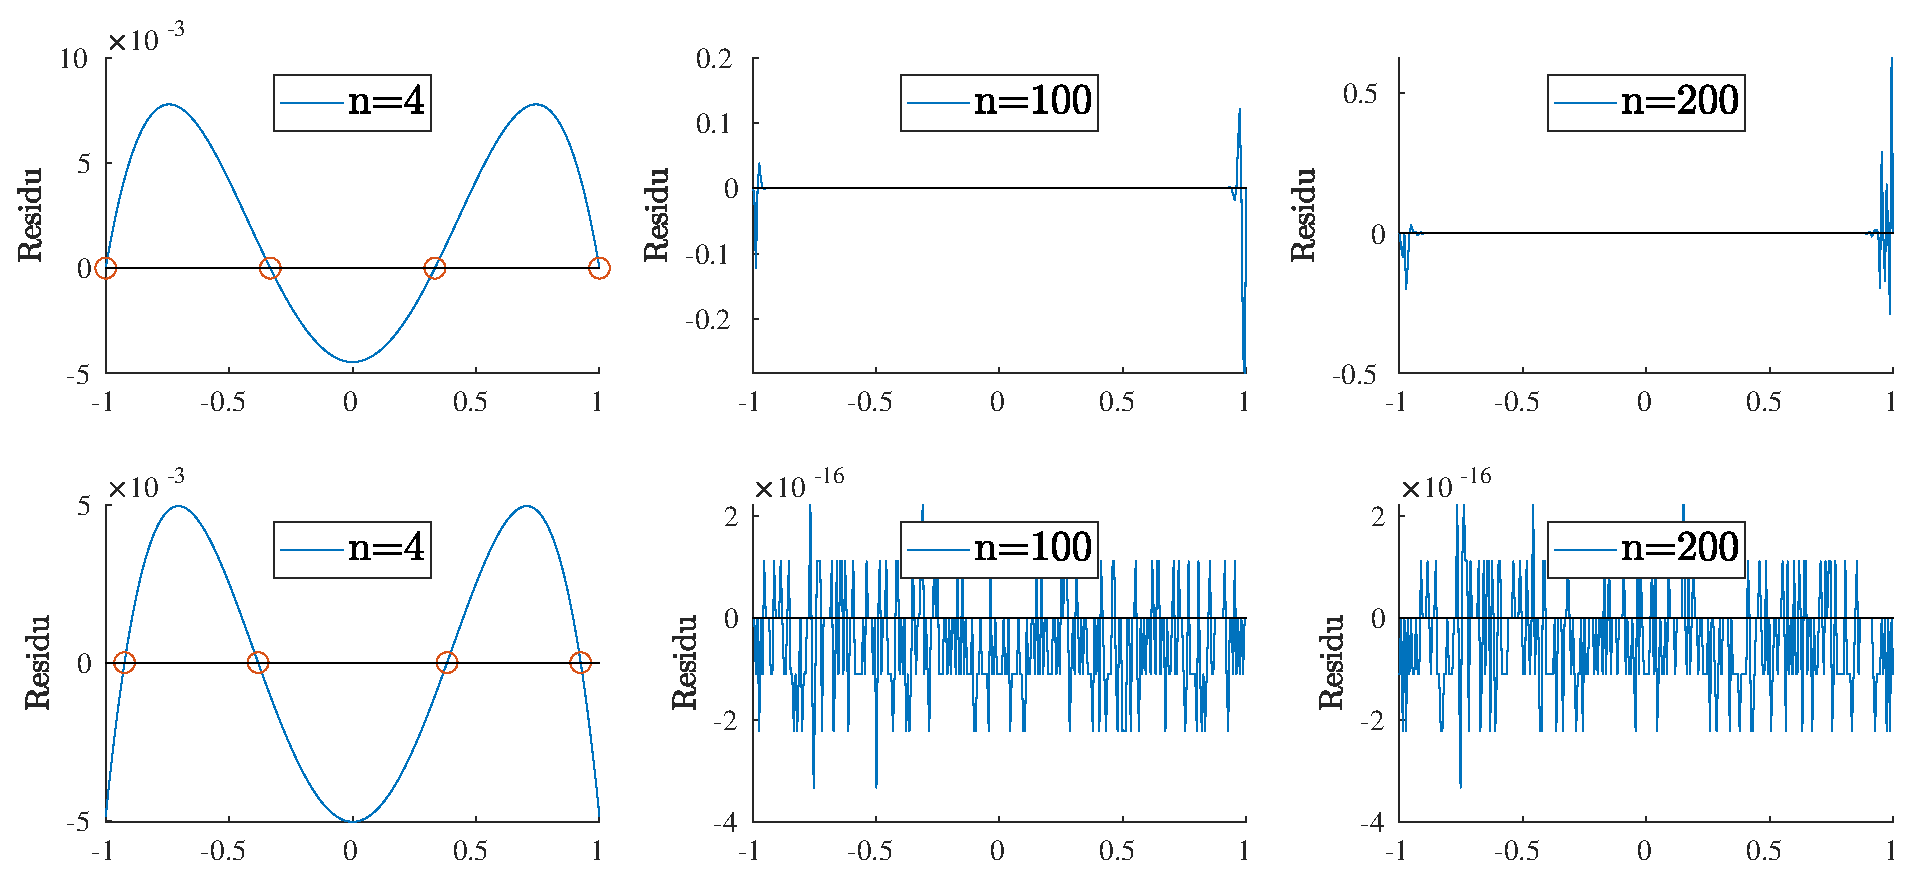
\includegraphics[width = \linewidth]{../Afbeeldingen/cos_heleFout.eps}
\caption{Fouten over het hele interval $[-1,1]$ voor verschillende waarden van $n$ voor de interpolatie van de cosinus functie. De bovenste rij figuren geeft de fout weer voor equidistante interpolatiepunten, terwijl de onderste rij figuren de fout voor Chebyshev-interpolatiepunten bevat. De interpolatiepunten zijn aangeduid in de eerste plot van elke reeks. Ze zijn weggelaten bij de andere plots om ze niet te onoverzichtelijk te maken.}
\label{fig:cosHeleFout}
\end{figure}

\begin{figure}
\centering
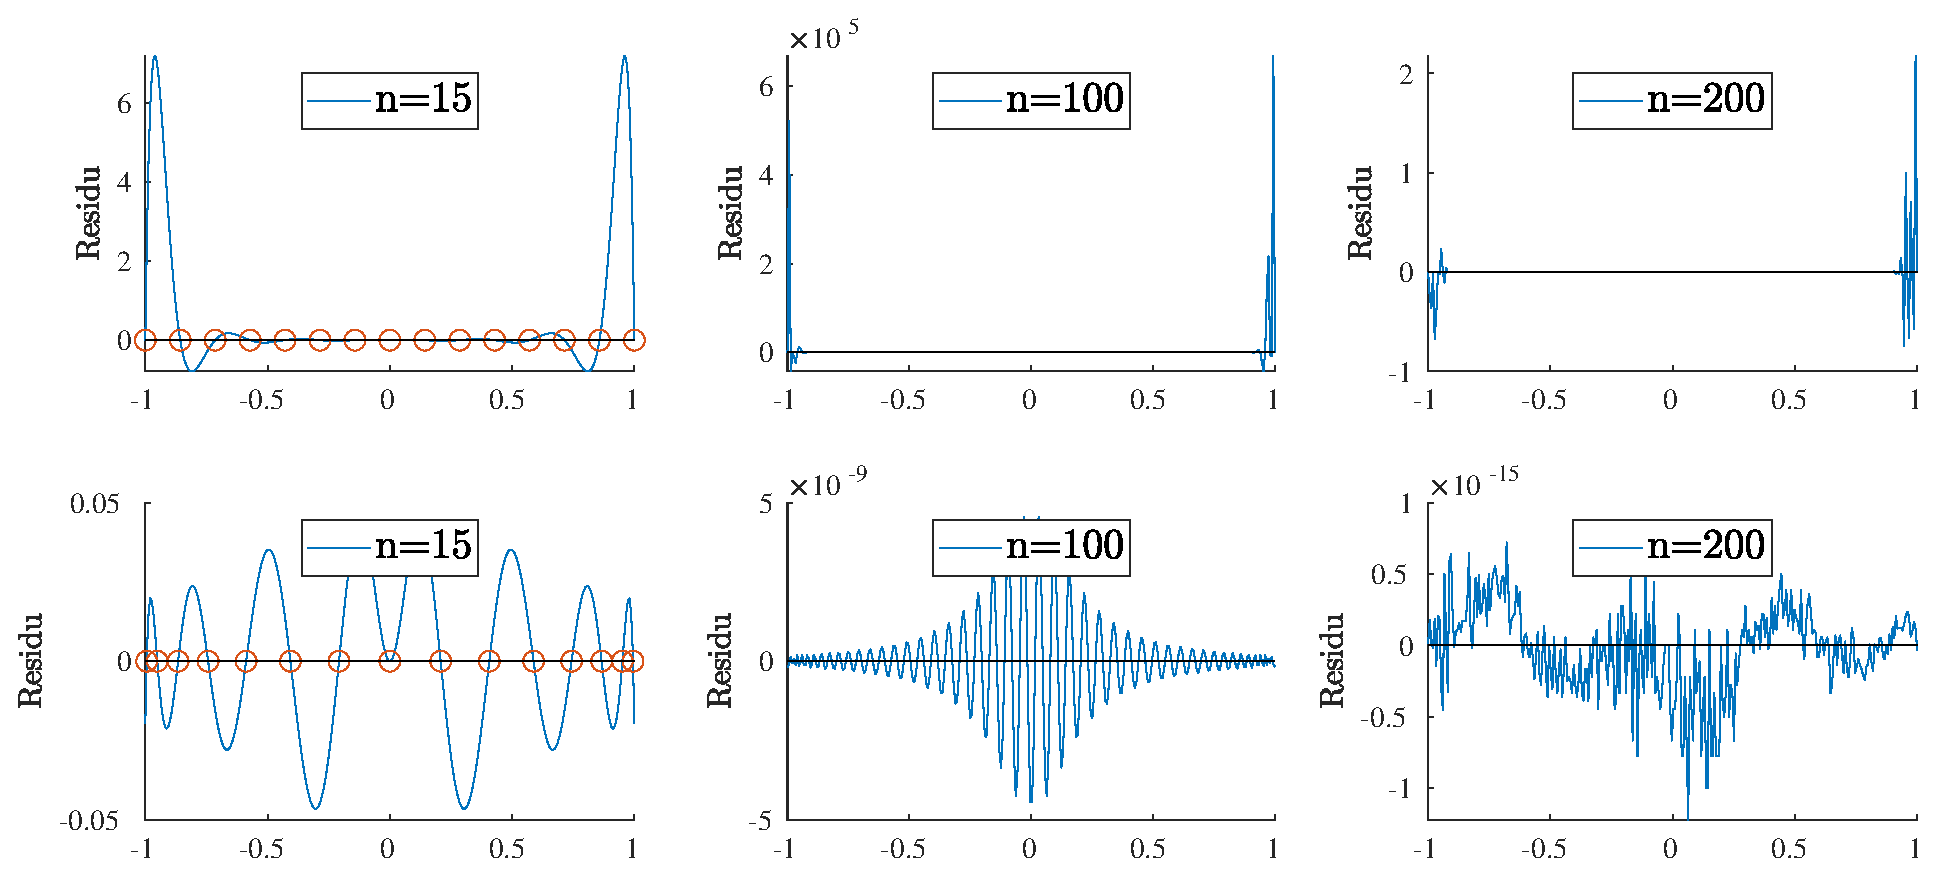
\includegraphics[width = \linewidth]{../Afbeeldingen/runge_heleFout.eps}
\caption{Fouten over het hele interval $[-1,1]$ voor verschillende waarden van $n$ voor de interpolatie van de runge functie. De bovenste rij figuren geeft de fout weer voor equidistante interpolatiepunten, terwijl de onderste rij figuren de fout voor Chebyshev-interpolatiepunten bevat. De interpolatiepunten zijn aangeduid in de eerste plot van elke reeks. Ze zijn weggelaten bij de andere plots om ze niet te onoverzichtelijk te maken.}
\label{fig:rungeHeleFout}
\end{figure}

\begin{figure}
\begin{subfigure}[b]{0.45\textwidth}
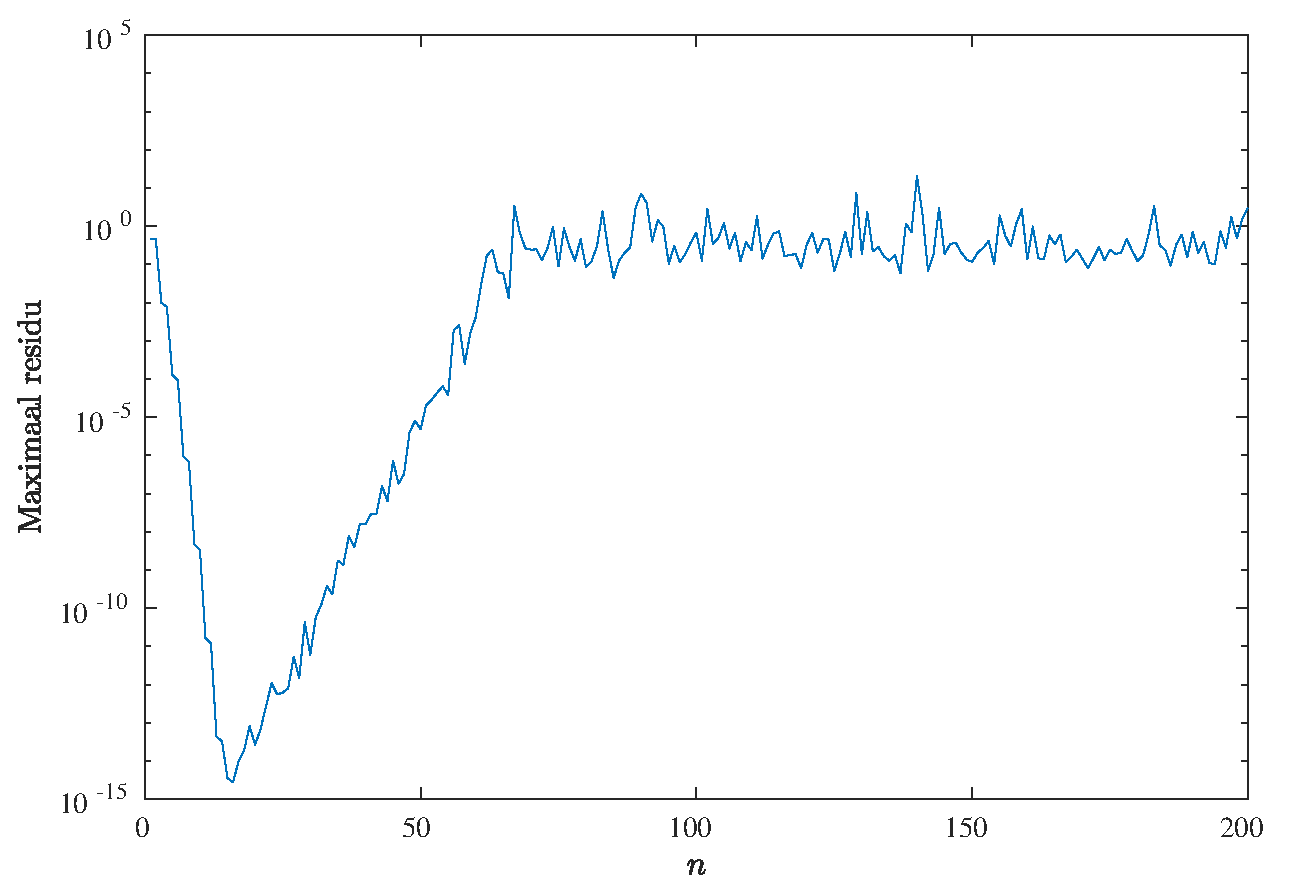
\includegraphics[width=\linewidth]{../Afbeeldingen/cos_equi_fout.eps}
\caption{Cosinus interpolatie met equidistante interpolatiepunten}
\end{subfigure}
\hfill
\begin{subfigure}[b]{0.45\textwidth}
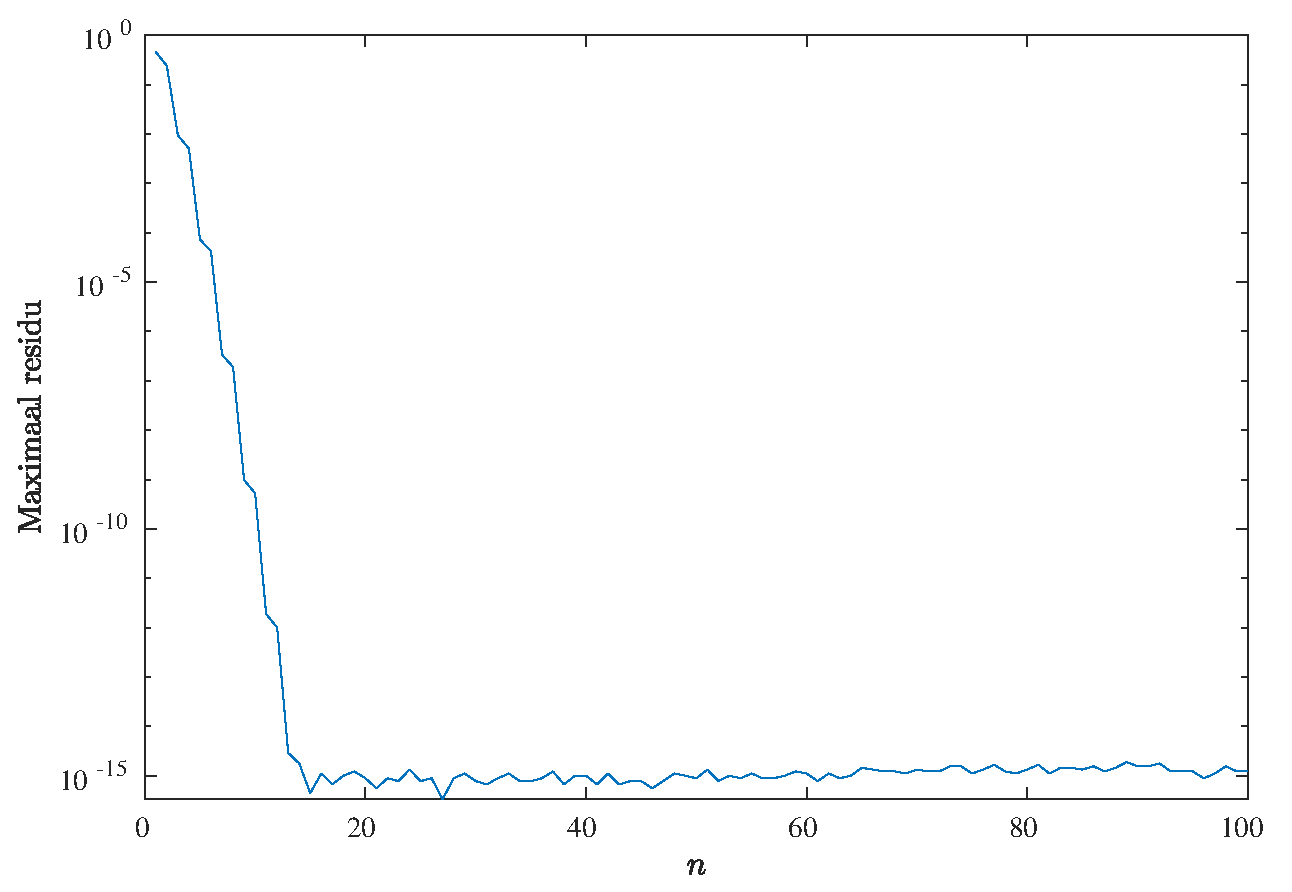
\includegraphics[width=\linewidth]{../Afbeeldingen/cos_nul_fout.eps}
\caption{Cosinus interpolatie met Chebyshev knooppunten}
\end{subfigure}
\caption{Fout bij interpolatie van de cosinus in functie van het aantal interpolatiepunten $n$}
\label{fig:cosFout}
\end{figure}

\begin{figure}
\begin{subfigure}[b]{0.45\textwidth}
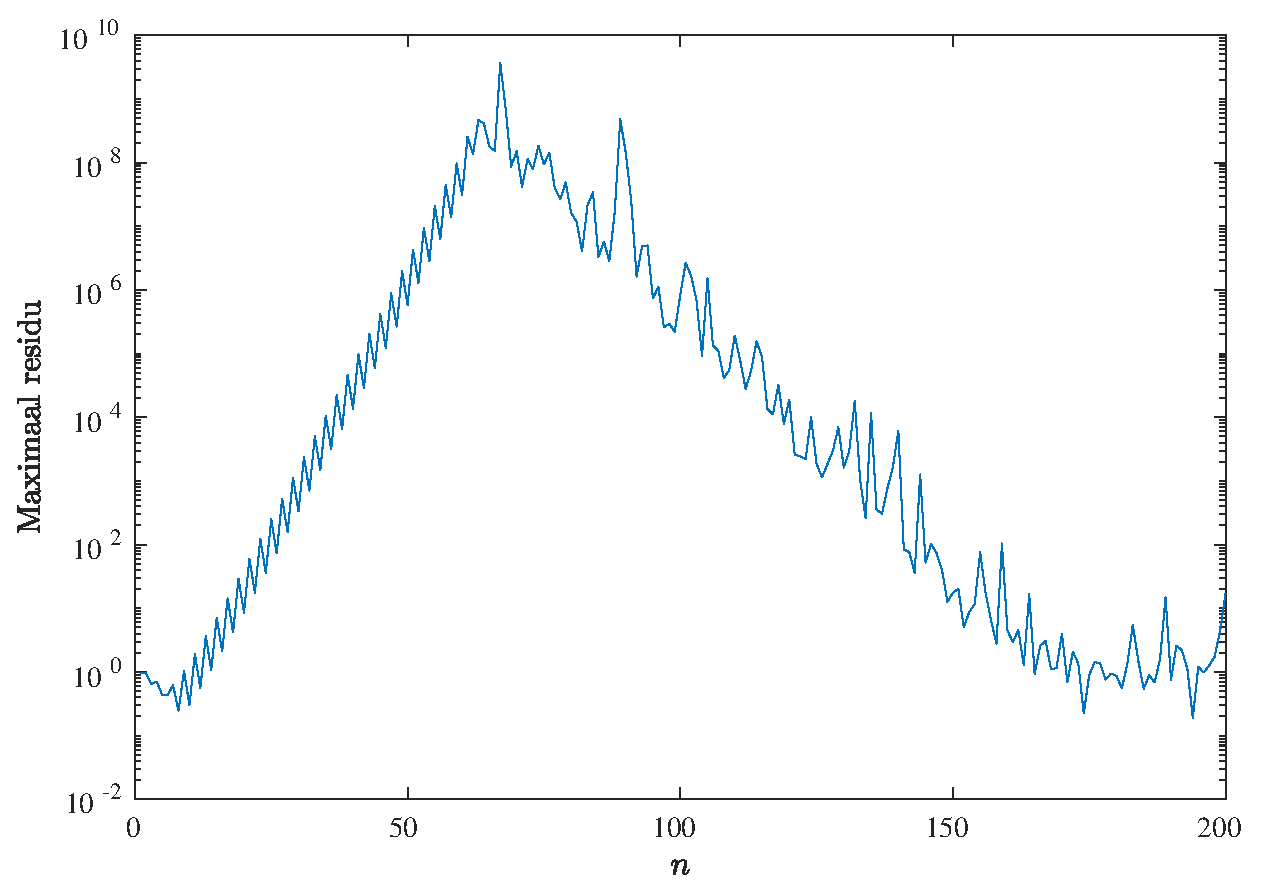
\includegraphics[width=\linewidth]{../Afbeeldingen/runge_equi_fout.eps}
\caption{Runge functie interpolatie met equidistante interpolatiepunten}
\end{subfigure}
\hfill
\begin{subfigure}[b]{0.45\textwidth}
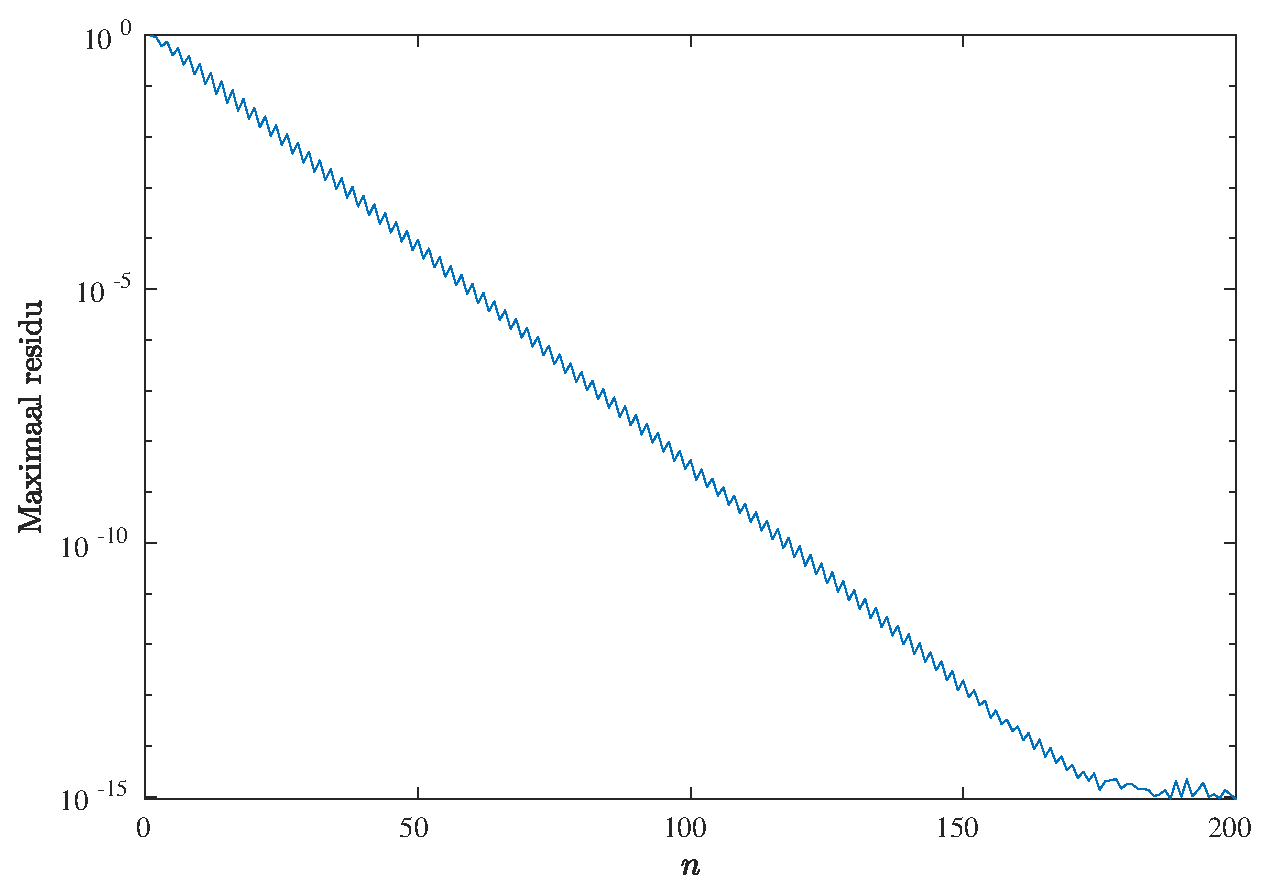
\includegraphics[width=\linewidth]{../Afbeeldingen/runge_nul_fout.eps}
\caption{Runge functie interpolatie met Chebyshev knooppunten}
\label{rungeNulFout}
\end{subfigure}
\caption{Fout bij interpolatie van de runge functie in functie van het aantal interpolatiepunten $n$.}
\label{fig:rungeFout}
\end{figure}

\begin{figure}
\begin{subfigure}[b]{0.45\textwidth}
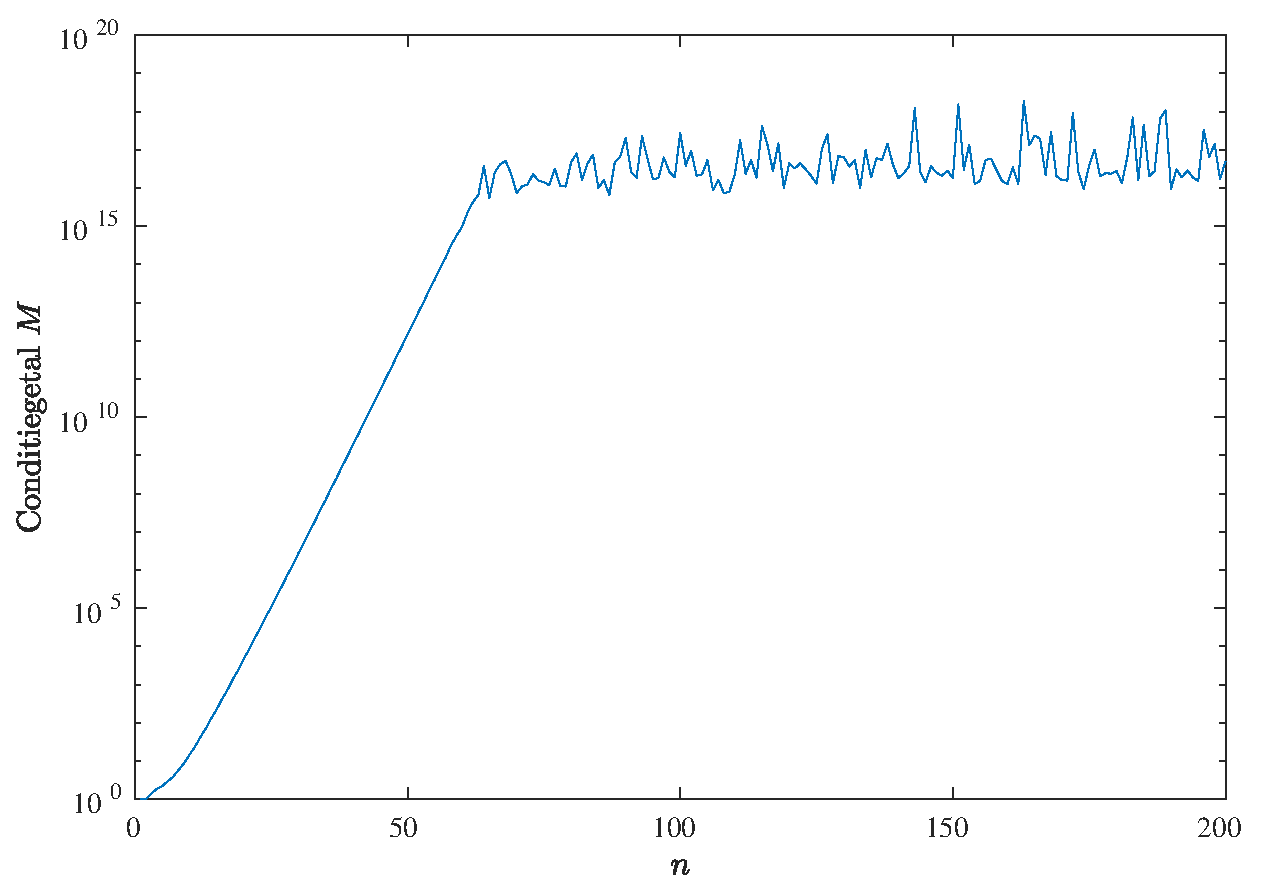
\includegraphics[width=\linewidth]{../Afbeeldingen/runge_equi_kappa.eps}
\caption{Conditiegetal bij equidistanteinterpolatiepunten}
\end{subfigure}
\hfill
\begin{subfigure}[b]{0.45\textwidth}
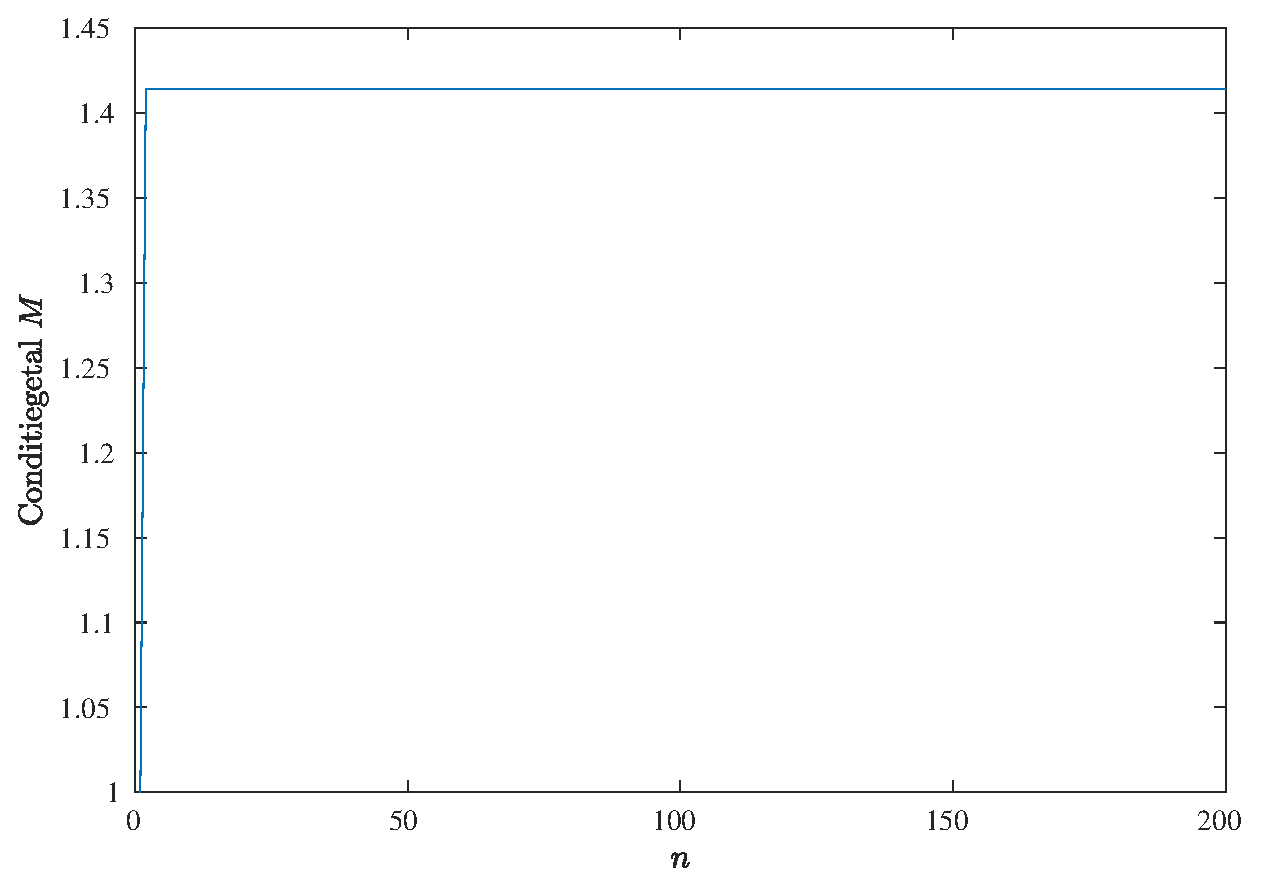
\includegraphics[width=\linewidth]{../Afbeeldingen/runge_nul_kappa.eps}
\caption{Conditiegetal bij interpolatie met Chebyshev knooppunten}
\end{subfigure}
\caption{Conditiegetal $\kappa$ van matrix $M$ in functie van het aantal interpolatiepunten~$n$}
\label{fig:kappa}
\end{figure}



\end{document}
